% Build: latexmk -lualatex main.tex   (quotes/ is generated by tools/leanquotes.py extract)
\documentclass[11pt]{article}
\usepackage[a4paper,margin=2.6cm]{geometry}
\usepackage{amsmath,amsthm,mathtools}
\usepackage{fontspec}
\usepackage{unicode-math}
\setmainfont{Libertinus Serif}
\setsansfont{Libertinus Sans}
\setmathfont{Libertinus Math}
\directlua{luaotfload.add_fallback("monofallback", {"STIX Two Math:mode=node;", "Noto Sans Mono:mode=node;"})}
\setmonofont{DejaVu Sans Mono}[Scale=0.82, RawFeature={fallback=monofallback}]
\usepackage{fvextra}
\fvset{breaklines=true, breakanywhere=true, fontsize=\footnotesize, frame=leftline, framesep=2mm, rulecolor=\color{black!35}}
\usepackage{xcolor}
\usepackage{tikz}
\usetikzlibrary{positioning,arrows.meta,fit}
\usepackage{booktabs,tabularx,longtable,array}
\usepackage{placeins}
\usepackage[hidelinks]{hyperref}
\usepackage{url}
\urlstyle{tt}
\usepackage[numbers,sort&compress]{natbib}
\usepackage{enumitem}
\setlist{itemsep=2pt,topsep=4pt}
\usepackage{microtype}

% ---- Lean references (all checked by tools/leanquotes.py check) ----
\newcommand{\lean}[1]{\nolinkurl{#1}}                 % a declaration name of the tree
\newcommand{\mathlib}[1]{\nolinkurl{#1}}              % a Mathlib name (not checked)
\newcommand{\leanloc}[2]{\nolinkurl{#1:#2}}           % file:line that starts a declaration
\newcommand{\leanlocx}[2]{\nolinkurl{#1:#2}}          % file:line inside a declaration
\newcommand{\leanquote}[1]{%
  \edef\lqfile{\directlua{tex.sprint(-2, (string.gsub("\luaescapestring{\detokenize{#1}}", "[.]", "-")))}}%
  \par\smallskip\noindent{\scriptsize\sffamily Source: \input{quotes/\lqfile.loc.tex}}%
  \VerbatimInput{quotes/\lqfile.lean}\smallskip}

% ---- status labels ----
\definecolor{tagc}{RGB}{40,90,150}
\newcommand{\sttag}[1]{{\color{tagc}\textsf{\small[#1]}}}
\newcommand{\stc}[1]{\sttag{classical}~\cite{#1}}
\newcommand{\stcs}{\sttag{classical, standard}}
\newcommand{\stl}[2]{\sttag{Lean: \leanloc{#1}{#2}}}
\newcommand{\stlx}[2]{\sttag{Lean: \leanlocx{#1}{#2}}}
\newcommand{\sta}[1]{\sttag{remark, item #1}}
\newcommand{\stad}{\sttag{remark}}
\newcommand{\sti}{\sttag{interpretation}}

\theoremstyle{definition}
\newtheorem{statement}{Statement}[section]
\theoremstyle{remark}
\newtheorem*{note}{Note}

\title{How the alpo.ge Lean source states a proof of the Riemann hypothesis:\\
an annotated map of its architecture}
\author{Yao Xu}
\date{Version 1.1.0, 21 November 2026}

\begin{document}
\maketitle

\begin{abstract}
A Lean~4 source tree of 175{,}187 files, published with a four-page note in November 2026,
contains a theorem \lean{riemannHypothesis} whose type is Mathlib's proposition
\mathlib{RiemannHypothesis}. This article explains, from the source text, how that theorem is
assembled. Short classical reductions bring the five exported theorems down to one proposition:
every Dirichlet $L$-function is non-zero on $\operatorname{Re}s>\tfrac12$, except at $s=1$ for
principal characters. The source links a one-sided bound for a weighted prime sum on sparse windows
of scales to zero-freeness, by a Landau-type criterion. Its arithmetic inputs include
Galois-cohomology length bounds over cyclotomic fields and declarations on Galois representations
attached to polarized regular algebraic cuspidal representations over CM fields, a form of the
local Langlands correspondence for $\mathrm{GL}_n$, and global theta lifts between unitary groups in
a stable range. Every claim below carries a source and a
status label, and a script extracts the Lean statements quoted from the alpo.ge source tree. As
reported in an independent verification record, the theorem \lean{riemannHypothesis}, with
Mathlib's definition, has been machine-checked by several independent checkers
(\S\ref{sec:verification}). What remains is the
reading of the mathematical argument by experts, and the agreement of Mathlib's definitions with the
classical ones.
\end{abstract}

\tableofcontents

\section{For the general reader}\label{sec:general}

The prime numbers $2,3,5,7,11,\dots$ thin out as they grow, and the prime number theorem says
how fast: up to $x$ there are about $x/\log x$ of them. The Riemann hypothesis would sharpen this
estimate. It bounds the difference between the prime count and the logarithmic integral
$\operatorname{Li}(x)=\int_2^x dt/\log t$ by a constant times $\sqrt{x}\log x$ for large $x$.
Riemann reformulated the question in 1859 in terms of a function $\zeta(s)$ of a
complex variable: the error is governed by the points where $\zeta$ vanishes, and the hypothesis
says that all of its non-obvious zeros lie on one vertical line, $\operatorname{Re}s=\tfrac12$.
Its generalization to Dirichlet $L$-functions controls primes in arithmetic progressions in the
same way.

In November 2026 a short note \cite{remark} reported the author's claim to have proved both
statements and linked to Lean~4 source for the argument \cite{alpotree,lean4}. Lean is a proof
assistant: a program that checks proof terms against its rules and the axioms they use. The Lean
source contains a line that
asserts the Riemann hypothesis, in exactly the form used by Lean's standard mathematical library
Mathlib \cite{mathlib2020}, together with about 175{,}000 files of supporting mathematics.

Two questions follow, and this article keeps them apart.
\begin{enumerate}
\item \emph{Does the program accept the proof?} This is a mechanical check. An independent
  verification record reports that the theorem, in Mathlib's form, has been machine-checked by
  several independent checkers; some runs were still going (\S\ref{sec:verification}). Such a check
  relies on the checkers and on Mathlib's definitions; whether those definitions agree with the
  classical ones is a separate question, on which \S\ref{sec:verification} reports one check.
\item \emph{What is the argument?} The source is far too large to read line by line. This article
  maps the statements and proof bodies supplied in the source, explains what the statements say,
  and traces how the main pieces connect. The reading of the argument by experts remains.
\end{enumerate}

In outline the argument runs as follows. The reductions in the source lead to the assertion that no
Dirichlet $L$-function vanishes on $\operatorname{Re}s>\tfrac12$, with $s=1$ excluded for principal
characters (where these $L$-functions have a pole). To exclude such zeros, the source bounds a weighted count of primes on a sequence of
ever-larger ranges of numbers (``windows''), and uses a classical positivity principle that turns a
one-sided bound of size $\sqrt{x}$ into the absence of zeros. The bound on the prime count in turn
is reduced to bounds on certain finite groups attached to cyclotomic fields (the fields generated by
roots of unity), and the source derives those bounds from statements modelled on some of the
deepest theorems of modern number theory: the correspondence between automorphic representations and Galois representations, and the
``theta correspondence'', which transports automorphic forms between groups of different sizes. For
a von Mangoldt sum of length $X$, the note suggests a chain of about $\sqrt{X}$ theta lifts, each
mimicking the ``multiplicity'' in Stepanov's elementary proof of the Riemann hypothesis for curves
over finite fields \sttag{remark, p.~1 and item 8} \stc{bombieri-stepanov}.

Each statement in this article carries a label saying where it comes from: a published theorem
(\sttag{classical}); a location in the Lean source (\sttag{Lean}, with module replay reported in
\S\ref{sec:verification}); the author's own description in
the note (\sttag{remark}); or our reading of the source (\sttag{interpretation}).

\section{What this article is, and how to read it}\label{sec:reading}

\paragraph{Object.} The object is the Lean~4 source tree \cite{alpotree} (Lean v4.33.1, Mathlib at
commit \texttt{0df444a3}), identified by the SHA-256 hash of its archive. It has 175{,}187
\texttt{.lean} files in ten libraries (Appendix~\ref{app:libraries}); the root file
\leanlocx{src/Main.lean}{1} exports five theorems. The accompanying note \cite{remark} gives a
timeline of twenty ideas (``items 1--20''), which \S\ref{sec:remark} maps to the source.

\paragraph{Status labels.} Every mathematical claim carries one of four labels.
\begin{description}[font=\normalfont]
\item[\sttag{classical}] a published theorem or a standard fact, with a citation.
\item[\sttag{Lean: file:line}] identifies a statement or definition in the source at this
  location. Where we discuss a proof body, the label refers to the body as written. The build,
  axiom check and kernel replay are in progress (\S\ref{sec:verification}).
\item[\sttag{remark, item $n$}] the author's own description in the note.
\item[\sttag{interpretation}] our reading: what a Lean statement means, or which published theorem
  it corresponds to. Lean declaration names are suggestive (the source has names such as
  \texttt{caraianiLocalGlobalDual} and \texttt{Green}) but they are not evidence; our
  interpretations rest on the quoted statements, and remain interpretations.
\end{description}
File paths are relative to the tree's \texttt{src/} directory and line numbers refer to the archive
with the hash above.

\paragraph{Quotations.} Lean statements are printed in framed boxes headed ``Source: file:line''.
Their text is produced by a script from the source, not typed: a theorem is quoted up to its
\texttt{:=} (the proof is elided as \texttt{:= …}), and a definition or structure is quoted with its
body. A checking script (Appendix~\ref{app:method}) regenerates every quotation and fails if any
box differs from the source, if a cited line does not start a declaration, or if a declaration name
in the text does not exist in the tree.

\paragraph{What the article does not do.} It does not judge whether the proof is correct; the
kernel check decides that. It does not trace the source to the bottom: the map follows the proof
from \texttt{Main.lean} downward for six to seven levels, until each branch reaches a named
theorem whose statement can be read on its own. The article compares the input statements reached
on those branches with results from the literature.

\paragraph{Notation.} $\chi$ and $\psi$ are Dirichlet characters; $L(s,\chi)$ is Mathlib's
\mathlib{DirichletCharacter.LFunction}, the meromorphic continuation of
$\sum_{n\ge1}\chi(n)n^{-s}$; $\Lambda$ is the von Mangoldt function; $\gamma$ is Euler's constant.
For a number field $E$, $\mathcal O_E$ is its ring of integers; for a CM field $E$, $E^+$ is its
maximal totally real subfield.

\section{The exported theorems and the classical reductions}\label{sec:top}

\subsection{What Main.lean states}

\texttt{Main.lean} imports two files: \texttt{Statements.lean}, which imports only Mathlib, and
\nolinkurl{Supplements/Kernels/MainTheoremsAll.lean} \stlx{src/Main.lean}{1}. Its first theorem has
Mathlib's proposition as its type:
\leanquote{riemannHypothesis}
\noindent Mathlib defines \mathlib{RiemannHypothesis} as: every $s\in\mathbb C$ with $\zeta(s)=0$,
$s\ne-2(n+1)$ for all $n\in\mathbb N$, and $s\ne1$ has $\operatorname{Re}s=\tfrac12$
\stc{mathlib2020}. (The definition explicitly excludes the pole $s=1$. Mathlib's
\mathlib{riemannZeta} is a total function and assigns a finite non-zero value there.) The tree restates this proposition in its
own words, and the second exported theorem proves the restatement with the same proof term, so the
two propositions must be definitionally equal for the file to compile:
\leanquote{RiemannZetaZerosOnLine}
\noindent The other three exported theorems are the generalized Riemann hypothesis for Dirichlet
$L$-functions in three forms: non-vanishing on $\operatorname{Re}s>\frac12$ (\lean{LFunction_ne_zero_of_half_lt_re},
\leanloc{src/Main.lean}{8}), zeros in the critical strip lie on the line for every character
(\leanloc{src/Main.lean}{10}) and for primitive characters (\leanloc{src/Main.lean}{12}). The first
of these is the statement everything else reduces to:
\leanquote{DirichletLNonvanishingRightOfHalf}

\subsection{One proposition carries the whole proof}

The four theorems in \texttt{Supplements/Kernels/MainTheorems.lean} that \texttt{Main.lean} re-exports
all take a single input, \lean{allChi}:
\leanquote{allChi}
\leanquote{rhOfAll}
\noindent where \lean{UpperTheory.EveryCharacter} is, word for word, the proposition
\lean{DirichletLNonvanishingRightOfHalf} again:
\leanquote{UpperTheory.EveryCharacter}

\begin{statement}[Every character]\label{st:every}
For every $N\ge1$, every Dirichlet character $\chi$ modulo $N$ and every $s$ with
$\operatorname{Re}s>\frac12$, except $\chi=1$ together with $s=1$, one has $L(s,\chi)\neq0$.
\stl{src/Development/AutomorphicArithmetic/CharacterBoxes/EveryCharacter.lean}{13}
\end{statement}

The rest of the traced source supplies the proof body of Statement~\ref{st:every}, the theorem
\lean{UpperTheory.FinalTheorems.everyCharacter} (\S\ref{sec:architecture}). The reductions from it
to the five exported theorems are short and use only Mathlib.

\subsection{The reductions}

\begin{enumerate}
\item \emph{Riemann hypothesis.} \lean{Formalism.VW.rh_of_every} specializes
  Statement~\ref{st:every} to the trivial character modulo $1$, whose $L$-function is $\zeta$
  (Mathlib's \mathlib{LFunction_modOne_eq}), and passes to \lean{Formalism.VW.rh_of_right}:
  \leanquote{Formalism.VW.rh_of_right}
  For a non-trivial zero $\rho$ with $\operatorname{Re}\rho<\frac12$, the proof first excludes
  $\rho=0$ using $\zeta(0)=-\frac12$. It then evaluates the functional equation
  $\zeta(1-s)=2(2\pi)^{-s}\Gamma(s)\cos(\pi s/2)\zeta(s)$ (Mathlib's \mathlib{riemannZeta_one_sub})
  at $s=1-\rho$, where the factors $2(2\pi)^{-s}$, $\Gamma(s)$ and $\cos(\pi s/2)$ are non-zero: a
  vanishing cosine in this range would force $\rho=0$ or a negative even integer
  \stl{src/Formalism/GammaFactorNonvanishing/RhOfRight.lean}{5} \stcs~\cite{davenport}.
\item \emph{Primitive characters, critical strip.} \lean{Formalism.VW.critLine}
  \stl{src/Formalism/GammaFactorNonvanishing/CritLine.lean}{11} does the same with the functional
  equation of the completed $L$-function of a primitive character, which relates $\chi$ at $s$ to
  $\chi^{-1}$ at $1-s$ (Mathlib's \mathlib{IsPrimitive.completedLFunction_one_sub}); the
  archimedean factor $\Gamma_{\mathbb R}(s+\kappa)$, $\kappa\in\{0,1\}$, is non-zero for
  $\operatorname{Re}s>0$ (\lean{Formalism.VW.gammaFactor_ne_zero},
  \leanloc{src/Formalism/GammaFactorNonvanishing/CritLine.lean}{6}).
\item \emph{All characters, critical strip.} \lean{Claim.strip}
  \stl{src/Development/AutomorphicArithmetic/CharacterBoxes/ClaimStrip.lean}{59} first passes from
  $\chi$ to the primitive character $\chi^\ast$ inducing it: in $0<\operatorname{Re}s<1$,
  $L(s,\chi)=L(s,\chi^\ast)\prod_{p\mid N}(1-\chi^\ast(p)p^{-s})$ and the Euler factors do not vanish
  because $|\chi^\ast(p)p^{-s}|<1$ (\lean{Claim.prim_zero}, \lean{Claim.factor_ne_zero}).
\item \emph{The statement for $\zeta$ in Mathlib's form} also follows directly (\lean{Claim.zeta},
  \leanloc{src/Development/AutomorphicArithmetic/CharacterBoxes/ClaimStrip.lean}{75}), using
  $\zeta(s)\ne0$ for $\operatorname{Re}s\ge1$ (Mathlib's \mathlib{riemannZeta_ne_zero_of_one_le_re}).
\end{enumerate}

These steps are the textbook passage from ``no zeros in $\operatorname{Re}s>\frac12$'' to ``all
non-trivial zeros on the line'' \stcs~\cite[Ch.~8--9]{davenport}. A second, parallel reduction,
\lean{UpperTheory.riemannHypothesis_of_everyCharacter}
\stl{src/Development/AutomorphicArithmetic/CharacterBoxes/RiemannHypothesisOfEveryCharacter.lean}{215},
is used by \lean{UpperTheory.FinalTheorems.riemannHypothesis} but not by \texttt{Main.lean}.
The kernel files \texttt{MainTheoremsAll.lean} and \texttt{MainTheoremsCritical.lean} (two and four
lines) state no theorem; they only import four further files on small class numbers.

\section{The architecture below Statement~\ref{st:every}}\label{sec:architecture}

\subsection{The last step}

The file \texttt{CharacterBoxes/MainConclusion.lean} (14 lines) proves Statement~\ref{st:every}:
\leanquote{UpperTheory.FinalTheorems.everyCharacter_of_row}
\leanquote{UpperTheory.FinalTheorems.everyCharacter}
\noindent The first theorem takes one hypothesis, a proposition \lean{UpperTheory.GalStar.Row0b}
about Galois representations (\S\ref{sec:galois}), and uses it three times: twice inside a structure
of ``literature statements'' and once to produce a window bound \lean{UpperTheory.Top.VWin}
(\S\ref{sec:window}). The second theorem discharges the hypothesis with a theorem of the tree,
\lean{UpperTheory.Gal.Int.galoisLocalGlobalStrong_recParameter}.

\subsection{How the literature fields are supplied}

The structure has three fields:
\leanquote{UpperTheory.LiteratureTheorems.OpenLiteratureStatements}
\noindent The first and third fields are the same proposition \lean{UpperTheory.One.M.Row}, which
unfolds to \lean{UpperTheory.GalStar.Row0b} with the local Langlands notion \lean{UpperTheory.Zero.LLC.IsRecT}
\stl{src/Development/AutomorphicArithmetic/Foundations/UnitarySphericalFixing/SatakeParameters/RecT.lean}{6};
the second is the local Langlands correspondence \lean{UpperTheory.Zero.LLC.RecTExists}
(\S\ref{sec:llc}). At \leanlocx{src/Development/AutomorphicArithmetic/CharacterBoxes/MainConclusion.lean}{8}
the structure is filled with $\langle h,\ \texttt{recTExists},\ h\rangle$, where $h$ is the
hypothesis of the first theorem and \lean{UpperTheory.Zero.LLC.recTExists} is a theorem of the tree.

The file declaring this structure contains 195 declarations taking
\texttt{O : OpenLiteratureStatements}. The names of 176 end in \texttt{\_of\_literature}, and many
name published results (Howe duality, the Siegel--Weil formula, the Rallis inner product formula,
Casselman--Wallach, Bernstein--Zelevinsky, Chebotarev, Poitou--Tate, and so on). The textual
dependency check (Appendix~\ref{app:method}) finds 13 declarations that reach a field of
\texttt{O}, directly or through another declaration in the file; for instance,
\lean{UpperTheory.LiteratureTheorems.local_langlands_recT_exists_of_literature} returns the field
\texttt{O.localLanglandsExists}. The other declarations cite results proved elsewhere in the tree.
For example, the body of
\leanquote{UpperTheory.LiteratureTheorems.logDerivOne}
\noindent (elided in the quotation) is \lean{GlobalTheory.LogDerOneProof.logDerOne_holds}. The
final construction supplies the first and third fields with the same Galois-representation
declaration and the middle field with \lean{UpperTheory.Zero.LLC.recTExists}.

\subsection{The map}

Figure~\ref{fig:top} shows the top of the proof. Arrows point from a statement to the statements
its proof uses. The left column is the analytic half (\S\ref{sec:analytic}); the right column is the
automorphic half (\S\ref{sec:window}--\ref{sec:automorphic}); \S\ref{sec:connection} explains the
crossings.

\begin{figure}[ht]
\centering
% Dependency diagram of the top levels (names abbreviated; full names and file:line in the text).
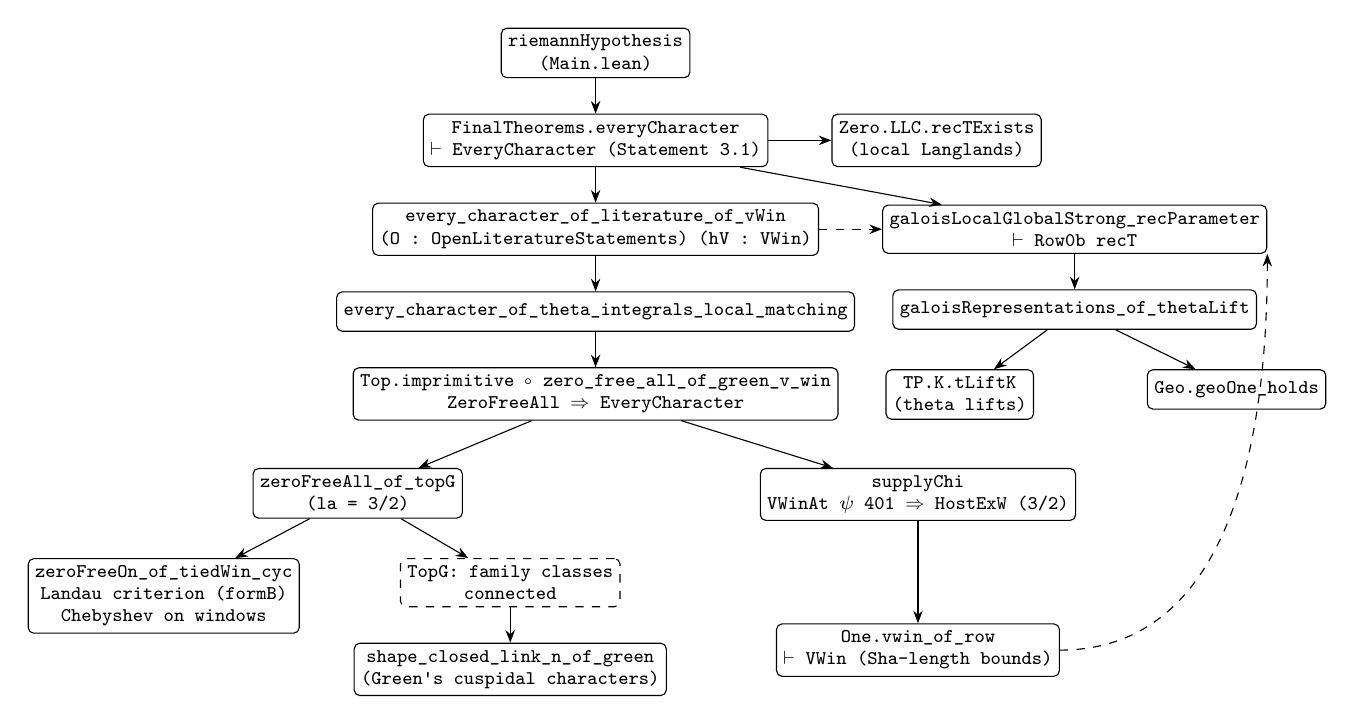
\begin{tikzpicture}[
  every node/.style={font=\scriptsize\ttfamily, align=center},
  thm/.style={draw, rounded corners=2pt, inner sep=2.5pt, minimum height=5mm},
  df/.style={draw, dashed, rounded corners=2pt, inner sep=2.5pt, minimum height=5mm},
  ->, >={Stealth[length=1.6mm]}, node distance=4.5mm and 6mm]
\node[thm] (rh) {riemannHypothesis\\(Main.lean)};
\node[thm, below=of rh] (every) {FinalTheorems.everyCharacter\\$\vdash$ EveryCharacter (Statement 3.1)};
\node[thm, below=of every] (lit) {every\_character\_of\_literature\_of\_vWin\\(O : OpenLiteratureStatements) (hV : VWin)};
\node[thm, below=of lit] (theta) {every\_character\_of\_theta\_integrals\_local\_matching};
\node[thm, below=of theta] (imp) {Top.imprimitive $\circ$ zero\_free\_all\_of\_green\_v\_win\\ZeroFreeAll $\Rightarrow$ EveryCharacter};
\node[thm, below left=6mm and -14mm of imp] (topg) {zeroFreeAll\_of\_topG\\(la = 3/2)};
\node[thm, below left=5mm and -6mm of topg] (landau) {zeroFreeOn\_of\_tiedWin\_cyc\\Landau criterion (formB)\\Chebyshev on windows};
\node[df, below right=5mm and -8mm of topg] (topgdef) {TopG: family classes\\connected};
\node[thm, below right=6mm and -10mm of imp] (supply) {supplyChi\\VWinAt $\psi$ 401 $\Rightarrow$ HostExW (3/2)};
\node[thm, below=of topgdef] (green) {shape\_closed\_link\_n\_of\_green\\(Green's cuspidal characters)};
\node[thm, below=13mm of supply] (vwin) {One.vwin\_of\_row\\$\vdash$ VWin (Sha-length bounds)};
\node[thm, right=8mm of lit] (row) {galoisLocalGlobalStrong\_recParameter\\$\vdash$ Row0b recT};
\node[thm, below=of row] (galth) {galoisRepresentations\_of\_thetaLift};
\node[thm, below left=5mm and -18mm of galth] (tlift) {TP.K.tLiftK\\(theta lifts)};
\node[thm, below right=5mm and -14mm of galth] (geo) {Geo.geoOne\_holds};
\node[thm, right=8mm of every] (llc) {Zero.LLC.recTExists\\(local Langlands)};
\draw (rh) -- (every);
\draw (every) -- (lit);
\draw (lit) -- (theta);
\draw (theta) -- (imp);
\draw (imp) -- (topg);
\draw (imp) -- (supply);
\draw (topg) -- (landau);
\draw (topg) -- (topgdef);
\draw (topgdef) -- (green);
\draw (supply) -- (vwin);
\draw (every) -- (row);
\draw (every.east) -- (llc);
\draw (row) -- (galth);
\draw (galth) -- (tlift);
\draw (galth) -- (geo);
\draw[dashed] (vwin.east) to[out=0, in=-90] (row.south east);
\draw[dashed] (lit.east) -- (row.west);
\end{tikzpicture}

\caption{The top of the proof of \lean{riemannHypothesis}. Boxes are Lean declarations
(abbreviated); solid boxes are theorems, dashed boxes are definitions. Every node is quoted or cited
with file:line in the text.}
\label{fig:top}
\end{figure}

\section{The analytic half: from prime sums on windows to zero-free half-planes}\label{sec:analytic}

This section follows the left column of Figure~\ref{fig:top}. Its result is that
Statement~\ref{st:every} follows from three inputs for each primitive character $\psi$: a
Landau-type criterion and a conditional square-root bound, both proved in the tree for every
``level'', and the existence of suitable families of auxiliary data on windows, which the
automorphic half supplies (\S\ref{sec:window}, \S\ref{sec:automorphic}).

\subsection{Primitive characters}

The analytic half works with primitive characters, packaged as a structure, and with the
proposition that all of their $L$-functions are zero-free on $\operatorname{Re}s>\frac12$:
\leanquote{Formalism.HC.PChar}
\leanquote{Formalism.HC.PChar.ZeroFreeAbove}
\leanquote{Formalism.HC.ZeroFreeAll}
\noindent Here \lean{Formalism.HC.ZeroFreeOn} \texttt{Q} requires \texttt{ψ.ZeroFreeAbove (1/2)} for
every \texttt{ψ} with \texttt{Q ψ} \stl{src/Formalism/SharpRestriction/RamificationFrobenius/TotientGaloisClasses/ExplicitFormulaErrorOfHostConditions.lean}{14}.
The passage back to all characters is the Euler-factor argument of \S\ref{sec:top} once more:
\leanquote{UpperTheory.Top.imprimitive}

\begin{note}
\lean{Formalism.HC.ZeroFreeAll} includes the trivial character modulo $1$ at $s=1$, where Mathlib's
$L$-function is \mathlib{riemannZeta} evaluated at its pole, a conventional finite value. The
statement therefore contains the assertion that this value is non-zero, which holds for Mathlib's
value (\S\ref{sec:top}). Statement~\ref{st:every}
excludes the pair ($\chi=1$, $s=1$) explicitly. \sti
\end{note}

\subsection{The prime sum}

The central analytic quantity is a weighted von Mangoldt sum with its expected main term removed:
\leanquote{Formalism.Sz}
\leanquote{Formalism.Gz}
\noindent That is,
\[
  S(x)=\sum_{n\le x}\Lambda(n)\Bigl(\frac{x}{n}-1\Bigr),\qquad
  G(x)=S(x)-x\log x+(1+\gamma)x .
\]
This is exactly the expression of remark item 5 \sta{5}. Its meaning is classical. Writing
$S(x)=\int_1^x\sum_{n\le t}\Lambda(n)n^{-1}\,dt$ and applying Perron's formula with the kernel
$x^{w}/(w(w-1))$ gives
\[
  S(x)=\frac1{2\pi i}\int_{(c)}\Bigl(-\frac{\zeta'}{\zeta}(w)\Bigr)\frac{x^{w}}{w(w-1)}\,dw\qquad(c>1).
\]
The double pole at $w=1$ contributes $x\log x-(1+\gamma)x$, which is precisely the term removed in
$G$. At $w=0$ the residue is $\log(2\pi)$. The non-trivial and trivial zeros give, for $x>1$,
\[
  G(x)=\log(2\pi)-\sum_{\rho}\frac{x^{\rho}}{\rho(\rho-1)}-\sum_{k\ge1}\frac{x^{-2k}}{2k(2k+1)},
\]
with non-trivial zeros counted with multiplicity. The zero sum converges absolutely and the
trivial-zero sum is $O(x^{-2})$ \stcs~\cite[Ch.~17]{davenport}\cite[Ch.~5]{iwaniec-kowalski}.
So $G(x)=O(x^{1/2})$ under the Riemann hypothesis, while a zero with real part $\beta>\frac12$
forces oscillations of size $x^{\beta}$. The tree uses twisted versions as well:
\leanquote{Formalism.HC.An.gChi}
\noindent For a non-principal character and $y\ge1$, the two terms are the weighted sum
$\sum_{n\le y}\chi(n)\Lambda(n)(y/n-1)$ and $y\,(L'/L)(1,\chi)$
\stl{src/Formalism/SharpRestriction/RamificationFrobenius/TotientGaloisClasses/Analytic.lean}{18}
\stl{src/Formalism/SharpRestriction/RamificationFrobenius/TotientGaloisClasses/Analytic.lean}{11}.
The latter cancels the residue contribution at $w=1$ \sti. A \emph{level} \lean{Formalism.HC.Level}
is a finite set \texttt{Λ.KEPT} of primitive characters with a natural number \texttt{o} and an
optional distinguished character \texttt{psK}. Its prime sum adds to $G$ the weighted real parts of
these twisted sums and their corrections, over the non-principal kept characters:
\leanquote{Formalism.HC.Level.Gm}
\noindent with weight $1$ for the distinguished character and $(3o+1)^{-1}$ for the others
\stl{src/Formalism/SharpRestriction/RamificationFrobenius/TotientGaloisClasses/ExplicitFormulaErrorOfHostConditions.lean}{36}.
The level used for $\psi$ is \lean{Formalism.HC.Level.cyc} $\psi$, built from the cyclic group
generated by $\psi$ \stl{src/Formalism/SharpRestriction/RamificationFrobenius/TotientGaloisClasses/ExplicitFormulaErrorOfHostConditions.lean}{121}.

\subsection{The Landau-type criterion on windows}

A set of reals \emph{has windows at scale} $\lambda$ if it contains intervals $[Y,Y^{\lambda}]$ with
$Y$ arbitrarily large:
\leanquote{Formalism.HC.HasWindows}
\noindent The criterion asserts that a one-sided bound $\Lambda.\mathrm{Gm}(x)\le x^{\theta}$ on such
windows excludes zeros to the right of $\theta$:
\leanquote{Formalism.HC.Level.FormBAt}
\noindent It is proved for every level and every $\lambda>1$:
\leanquote{UpperTheory.Comparison₂.formB}
\noindent The proof transports the level to a weighted family of characters with the same prime sum
and the same zero-freeness (\lean{UpperTheory.Comparison₂.level_family},
\leanloc{src/Development/AutomorphicArithmetic/PrimitiveCosets/LevelFamily.lean}{41}) and applies
\leanquote{Deduction.zeroFree_of_rpow_window}

\begin{statement}[Landau-type criterion]\label{st:landau}
Let $F$ be a finite family of positively weighted Dirichlet characters in which any principal
character has modulus $1$ (a level becomes one through
\lean{UpperTheory.Comparison₂.level_family}). Fix $0<\theta<1$ and $\delta>0$. Suppose there is a
real $C$ such that for every $Y_0$ there is $Y\ge Y_0$ with $\mathrm{Gm}_F(y)\le C\,y^{\theta}$ for
all $y\in[Y,Y^{1+\delta}]$. Then each $L$-function in $F$ is non-zero for
$\operatorname{Re}s>\theta$, in Mathlib's total-function convention.
\stl{src/Development/AutomorphicArithmetic/DedekindLFunctions/LandauTheorems/ZeroFreeOfRpowWindow.lean}{11}
\end{statement}

Two features distinguish this from the textbook statement. First, the bound is one-sided. In the
classical theory a one-sided bound excludes zeros through positivity: by Landau's theorem, a
Dirichlet series or Mellin transform of a function of constant sign is analytic to the right of a
real singularity. Applied to $C x^{\theta}-G(x)$, a one-sided bound on $G$ pushes every pole coming
from a zero $\rho$ to $\operatorname{Re}\rho\le\theta$, provided no real singularity intervenes
\stcs~\cite[Ch.~1 and~15]{montgomery-vaughan}. Second, the bound is required only on windows
$[Y,Y^{1+\delta}]$, not for all large $y$. We have not read the proof of
Statement~\ref{st:landau} (the lemma \lean{Deduction.lemmaL} that it calls) and do not know which
positivity it uses; this is question~Q4 in the list for outside experts.

\subsection{The conditional square-root bound}

The bound fed into Statement~\ref{st:landau} comes from auxiliary \emph{families}. A family
\texttt{Fm} (of type \lean{Formalism.BasicNotions.Fam} $\varepsilon$, or its variant
\lean{Formalism.MainNotions.FamP}) carries a set of windows \texttt{Win} and, for each $x$,
an index set of local and global data. The square-root bound is stated relative to a predicate
\texttt{Tied} on families:
\leanquote{Formalism.HC.ChebyshevInequalityOnWindows}
\noindent and the input needed at a given scale is the existence of level-compatible
(\texttt{EFamC}), tied families with windows:
\leanquote{Formalism.HC.ChebyshevInequalityAtWindowScale}
\noindent With $\varepsilon$ free, these give zero-freeness on $\operatorname{Re}s>\frac12$:
\leanquote{Formalism.HC.zeroFreeOn_of_tiedWin_cyc}
\noindent (In \lean{Formalism.HC.level_of_tiedWin} the proof picks $\varepsilon$ with
$(e_D+e_L+7)\varepsilon$ below half the distance from $\operatorname{Re}s$ to $\frac12$ and applies
the criterion with $\theta=\frac12+\frac12\min(\operatorname{Re}s-\frac12,\frac12)$
\stl{src/Formalism/SharpRestriction/RamificationFrobenius/TotientGaloisClasses/TopWin.lean}{68}.)

The first hypothesis holds for every level, with \texttt{Tied} the predicate
\lean{Formalism.MainNotions.ChainTied}:
\leanquote{UpperTheory.Comparison₂.level_gm_le_on_family_scales}
\noindent So, as written: for any level $\Lambda$ and $\varepsilon>0$, a family satisfying
\texttt{EFamC Λ} and \texttt{ChainTied} at all sufficiently large points of its window set has
$\Lambda.\mathrm{Gm}(x)\le x^{1/2+(e_D+e_L+7)\varepsilon}$ at all sufficiently large points of that
set. The difficulty is moved into producing level-compatible, chain-tied families. The predicate
\lean{Formalism.MainNotions.ChainTied}
\stl{src/Formalism/SharpRestriction/GlobalSchurBounds/TieGlobal.lean}{97} is a large compatibility
condition that ties the family's data at $x$ to: ranks and slopes $\mu$, $\mu_{\max}$ of lattices
(\texttt{TieLocal}), arithmetic data including the values \texttt{logDerivativeAtOne χ} of primitive
characters (\texttt{TieArith}), size data of an ``$L$-function chain''
(\texttt{LFunctionChainParameters.LChain.SizeData₂}) and error terms on windows (\texttt{ErrWindows}).
The slope vocabulary is that of Arakelov-theoretic slope inequalities, which remark item 13 names
(the Bost slope inequality) \sti~\stc{bost}. We have not unpacked this predicate.

\subsection{Where the families come from}

The remaining input is supplied for every $\psi$ by the following theorem, applied with
$\lambda=\frac32$:
\leanquote{UpperTheory.Top.zeroFreeAll_of_topG}
\noindent It has two hypotheses. The first is \lean{UpperTheory.Top.TopG}. For any $\lambda>1$, it
applies to a requirement \texttt{G} supplied by \texttt{HostExW λ G.req} whose class satisfies the
Galois-cohomology condition \lean{UpperTheory.Top.HypV}. It then supplies an eventually chain-tied
member of that class for each sufficiently small positive $\varepsilon$, with common exponents
$e_D,e_L$ (the class is ``connected''):
\leanquote{UpperTheory.Top.TopG}
\leanquote{UpperTheory.Top.FamilyClassConnected}
\noindent For the requirement \lean{UpperTheory.Top.GChi} $\psi$
\stl{src/Development/AutomorphicArithmetic/CharacterBoxes/Supply.lean}{42}, membership in the class
supplies the windows and level compatibility (\lean{UpperTheory.Top.eFamC_of_cls}); the requirement
combines an analytic condition at the cyclotomic level of $\psi$ with the Galois-cohomology bound
\lean{UpperTheory.Top.VVle} of \S\ref{sec:window}. The second input is
\texttt{HostExW λ (GChi ψ).req} for every primitive $\psi$. Both hypotheses are discharged in
\lean{UpperTheory.Top.zero_free_all_of_green_v_win}
\stl{src/Development/AutomorphicArithmetic/ThetaCorrespondence/ThetaPairLifts/ThirdPlaceSeries/TopPlug.lean}{12}:
\begin{itemize}
\item \lean{UpperTheory.Top.TopG} from Green's classification of cuspidal characters of finite
  general linear groups together with the theta-integral hypotheses (\S\ref{sec:thetaside}), through
  \lean{UpperTheory.Top.shape_closed_link_n_of_green}
  \stl{src/Development/AutomorphicArithmetic/ThetaCorrespondence/ThetaPairLifts/ThirdPlaceSeries/TopShape.lean}{33};
\item the supply from the window bound, through \lean{UpperTheory.Top.supplyChi}
  \stl{src/Development/AutomorphicArithmetic/CharacterBoxes/SupplyChi.lean}{8}:
  $\texttt{VWinAt}\ \psi\ 401\Rightarrow\texttt{HostExW}(3/2)\,(\texttt{GChi}\ \psi)\texttt{.req}$.
\end{itemize}

\paragraph{Summary of the analytic half.} For each primitive $\psi$, as written:
\[
\begin{aligned}
\underbrace{\text{\begin{tabular}{@{}c@{}}level-compatible, chain-tied\\families on windows\end{tabular}}}_{\text{TopG + supply}}
&\ \xRightarrow{\ \texttt{level\_gm\_le\_on\_family\_scales}\ }\
\Lambda.\mathrm{Gm}(x)\le x^{1/2+O(\varepsilon)}\text{ on windows}\\
&\ \xRightarrow{\ \text{Statement \ref{st:landau}}\ }\
L(s,\psi)\ne0\ (\operatorname{Re}s>\tfrac12).
\end{aligned}
\]

\section{The window bound: Galois cohomology over cyclotomic fields}\label{sec:window}

The supply hypothesis of \S\ref{sec:analytic} comes from one proposition, \lean{UpperTheory.Top.VWin},
which bounds Tate--Shafarevich groups of Tate twists over a family of abelian fields. It is the place
where the analytic half receives arithmetic input.

\subsection{The statement}

\leanquote{UpperTheory.Top.VWin}
\leanquote{UpperTheory.Top.VWinAt}
\noindent The auxiliary conditions are: a ``page'' size $2^{e}$ comparable with $x^{2+8\varepsilon}$,
\leanquote{UpperTheory.Top.PageN}
\noindent a pair of primes $q,d$ of prescribed size and congruence type,
\leanquote{UpperTheory.Top.WinPair}
\noindent the fields to which the bound applies,
\leanquote{UpperTheory.Top.IsChiField}
\noindent and the bound itself:
\leanquote{UpperTheory.Top.VAt}
\leanquote{UpperTheory.Top.VVle}

\subsection{What the bound says}

The groups are defined in \texttt{Formalism/GaloisCohomology/Statement.lean}. For a number field $F$,
a prime $\ell$ and the set $S$ of places of $F$ above $\ell$, an \lean{Formalism.GaloisCohomology.LData}
records the Galois group $G_S$ of the maximal extension unramified outside $S$, decomposition data at
$S$, and the $\ell$-adic cyclotomic character
\stl{src/Formalism/GaloisCohomology/Statement.lean}{54}. The coefficient module is
$\mathbb Q_\ell/\mathbb Z_\ell$ with $G_S$ acting through the cyclotomic character to the power
$-e$:
\leanquote{Formalism.GaloisCohomology.qzTw}
\noindent and \lean{Formalism.GaloisCohomology.Sha} is the kernel of localization at $S$ in
$H^1$ \stl{src/Formalism/GaloisCohomology/Statement.lean}{75}, measured by its
$\mathbb Z_\ell$-length:
\leanquote{Formalism.GaloisCohomology.shaLen}

\begin{statement}[Window bound, as stated]\label{st:vwin}
For every primitive character $\psi$, every $0<\varepsilon<\frac1{52}$ and every function
$e:\mathbb R\to\mathbb N$ satisfying $x^{2+8\varepsilon}\le 2^{e(x)}\le 2x^{2+8\varepsilon}$ for all
$x\ge1$, there are reals $J\ge1$ and $X_0$ such that for $X\ge X_0$ and every prime pair $(q,d)$ of the shape \texttt{WinPair}
$\varepsilon$ $X^{1/J}$, there is $Y\in[X^{1/J},X^{1/2}]$ such that for all $x\in[Y,Y^2]$ and every
number field $E$ of type \texttt{IsChiField} $\psi\ e(x)\ q\ d$:
\[
\sum_{\ell\in S}\log\ell\sum_{e=1}^{t-1}\operatorname{length}_{\mathbb Z_\ell}
\text{Ш}^1\bigl(G_{S_\ell}(E),\,\mathbb Q_\ell/\mathbb Z_\ell(-e)\bigr)\ \le\ \exp\bigl(x^{\varepsilon}/2\bigr),
\qquad t=\lfloor x^{401}\rfloor,
\]
The inequality holds for every finite set $S$ of primes and for every choice of an algebraic
closure and family of local data \texttt{LData}. Each indicated length is finite for every prime
$\ell$ and every $1\le e<t$.
\stl{src/Development/AutomorphicArithmetic/CharacterBoxes/ExistsPageN.lean}{44}
\end{statement}

The fields $E$ of type \texttt{IsChiField} are subfields of $\mathbb Q(\zeta_N)$, with $2^{e+2}$, the
conductor of $\psi$, $q$ and $d$ dividing $N$, cut out by the conditions $a\equiv\pm1\pmod{2^{e+2}}$,
$\psi(a)=1$ and $\bigl(\frac aq\bigr)=\bigl(\frac ad\bigr)=1$ on $a\in(\mathbb Z/N)^\times$. As $x$
grows, $e(x)$ grows like $(2+8\varepsilon)\log_2 x$, so these fields climb the cyclotomic
$\mathbb Z_2$-tower, twisted by $\psi$ and by two quadratic characters \sti. The note describes an
Iwasawa tower chosen by analogy with $\mathbb F_{q^n}/\mathbb F_q$ \sta{11} and a precise choice of
the tower \sta{19}; the classes in $H^1(\mathcal O_E[1/\ell],\mathbb Q_\ell/\mathbb Z_\ell(-e))$ that
cannot be removed by twisting, and a ``significant weakening of Vandiver'', are item 17 \sta{17}.
Statement~\ref{st:vwin} controls the $\log\ell$-weighted sum of lengths of the localization kernels
in these $H^1$ groups over primes $\ell$ and twists $1\le e<t$. We compare this localization-kernel
bound with item 17 \sti. How this relates to known results on these groups is question~Q5. (For background on Ш$^1$ and
Poitou--Tate duality see \cite[Ch.~VIII]{nsw}; for Vandiver's conjecture, \cite[§8.3]{washington}.)

\subsection{How the tree proves the window bound}

\leanquote{UpperTheory.One.vwin_of_row}
\noindent The proof goes through \lean{UpperTheory.One.Join.automorphic_window_of_inputs}
\stl{src/Development/AutomorphicArithmetic/AutomorphicVarieties/ModularityArgument/ThresholdArguments/DenseThresholdCases/TopMainZj.lean}{71}
and \lean{UpperTheory.V.v_window_of_literal_automorphy_n}, whose hypothesis is a structure of four
propositions:
\leanquote{GlobalTheory.Mem.LiteralAutomorphy.LiteratureRankNHypothesis}
\noindent These are filled from the Galois-representation theorem \lean{UpperTheory.GalStar.Row0b}
(through the structure \lean{UpperTheory.LiteratureTheorems.OpenImageCondition}, whose single field is
the same proposition), from the base-change theorem \lean{UpperTheory.BaseChangeIdentities.baseChangeN}
\stl{src/Development/AutomorphicArithmetic/Foundations/BaseChangeIdentities/DefiniteNHolds.lean}{5}
and from theorems of the tree on local representation theory, Galois cohomology and CM abelian
varieties. The final step is
\lean{UpperTheory.V.HV.DescentVanishingReductions.v_window_of_automorphy_csd_ss_mono_odd}
\stl{src/Development/AutomorphicArithmetic/AutomorphicVarieties/ModularityArgument/ThresholdArguments/DenseThresholdCases/WindowBoundOfLiteratureLevel.lean}{30},
and the next call is to
\lean{UpperTheory.V.HV.DescentVanishingReductions.published_hypotheses_from_patching_alt}, which
assembles the input record \lean{UpperTheory.V.Af.HypothesesH'}. The surrounding directory names
(\texttt{ModularityArgument}, \texttt{AutomorphyLifting}, \texttt{PatchingModules}) suggest a
Taylor--Wiles-style interpretation \sti; we have not traced it further.

\section{The automorphic half}\label{sec:automorphic}

Three deep inputs sit at the bottom of the right column of Figure~\ref{fig:top}. The source
supplies declarations and proof bodies for the three inputs discussed here. This section gives
their statements, the published results they resemble, and the proof references we traced.

\subsection{Galois representations for polarized cuspidal representations}\label{sec:galois}

\leanquote{UpperTheory.GalStar.Row0b}
\leanquote{UpperTheory.GalStar.PropsB}
\leanquote{GlobalTheory.ContraPair.PolarizedPair}

\begin{statement}[Galois representations, as stated]\label{st:row}
Let $E$ be a CM field, $\ell$ a prime, $\iota:\overline{\mathbb Q}_\ell\simeq\mathbb C$ and $a\ge1$. Let
$\pi$ be a regular algebraic cuspidal representation of $\mathrm{GL}_a$ over $E$
(\texttt{CuspSub E a}), and let $\chi$ be a Hecke character of $E^+$ with $\chi_v(-1)=(-1)^a$ at every
infinite place $v$. The polarization condition pairs $\pi$ twisted by
$(\chi\circ\mathrm N_{E/E^+})^{-1}$ with $\pi$ under the conjugated action. Then there exist a
continuous semisimple $r:G_E\to\mathrm{GL}_a(\overline{\mathbb Q}_\ell)$, an integer $\mathrm{wt}$
and multisets $\mathrm{HT}(\tau)$ with the following properties. At each finite place $w\nmid\ell$,
for each local correspondence $\mathrm{rc}$ satisfying the notion \texttt{Rc} and each local
component $\sigma$ of $\pi$, the Weil--Deligne parameters of $r$ and of
$\mathrm{rc}(\mathrm{algNorm}(\sigma))$, where \texttt{algNorm} twists $\sigma$ by
$|\det|^{(1-a)/2}$, have equal dimension. The structure \lean{UpperTheory.GalStar.AwayB} gives
their equality in its toral, zero-monodromy case, and equality of inertia characteristic polynomials
with zero monodromy under its specified tame hypotheses (field \texttt{away}). The multiset
$\mathrm{HT}(\tau)$ consists of $\frac{a-1}2$ minus the infinitesimal weights of $\pi$ at $\iota\tau$
(field \texttt{weights}), and conjugation of $\tau$ sends each weight $h$ to $\mathrm{wt}-h$ (field
\texttt{weights\_conj}). The field \texttt{above} adds conditional local crystalline, de Rham,
potentially semistable and Hodge--Tate compatibility conclusions.
\stl{src/Development/AutomorphicArithmetic/Foundations/GaloisRepresentations/TypeConditions/WeightsConjBis.lean}{69}
\end{statement}

\noindent The proposition used in the proof is \texttt{Row0b recT}, with \texttt{Rc} the local
Langlands notion of \S\ref{sec:llc}. In the literature, Galois representations attached to
regular algebraic, polarized (``essentially conjugate self-dual'') cuspidal representations of
$\mathrm{GL}_a$ over CM fields were constructed by Shin \cite{shin} and Chenevier--Harris
\cite{chenevier-harris}, building on Harris--Taylor \cite{harris-taylor}; local--global compatibility
at $w\nmid\ell$ (including monodromy) is due to Caraiani \cite{caraiani-duke}. For the terminology
of polarized representations see \cite{blggt}; the displayed sign condition is the one in
\texttt{PolarizedPair}. Statement~\ref{st:row} has the shape of this theorem \sti. Whether its
normalizations (the shift $\frac{a-1}2$, the twist \texttt{algNorm}, the conditions in
\texttt{AwayB} and on $\mathrm{rc}$) agree with the published statements is question~Q1.

The traced route uses a theta-lift input and an input supplied by
\lean{UpperTheory.Gal.Int.Geo.geoOne_holds}, through a weight-one geometric realization. The proof
is
\leanquote{UpperTheory.Gal.Int.galoisLocalGlobalStrong_recParameter}
\leanquote{UpperTheory.Gal.Int.galoisRepresentations_of_thetaLift}
\noindent and, one level down,
\lean{UpperTheory.Gal.Int.galoisLocalGlobal_of_geometry_lift}
\stl{src/Development/AutomorphicArithmetic/Foundations/GaloisRepresentations/IntegralStructures/Development.lean}{27}
combines three ingredients: a ``seed'' obtained from \lean{UpperTheory.Gal.Int.Geo.GeoOne}
(\lean{UpperTheory.Gal.Int.Div.seedFinOdd_of_geoOne}), congruences at odd finite level
(\lean{UpperTheory.Gal.Int.Cong.congFinOdd_of_ex}), and the theta lifts of \S\ref{sec:theta}.
\lean{UpperTheory.Gal.Int.Geo.GeoOne}
\stl{src/Development/AutomorphicArithmetic/Foundations/GaloisRepresentations/IntegralStructures/GeometricFlagBases/HodgeTrAt.lean}{79}
is a long statement: for odd $a$, an auxiliary imaginary quadratic datum $x^2=-d$, a non-split set of
places, and an automorphic subspace $U$ of a unitary group with prescribed local types. Under its
stated hypotheses, \texttt{GeoOne} supplies a representation with the required Satake data for each
eligible place away from $\ell$; the choice of representation is inside the quantifier over places.
It is proved as \lean{UpperTheory.Gal.Int.Geo.geoOne_holds}
\stl{src/Development/AutomorphicArithmetic/Foundations/GaloisRepresentations/IntegralStructures/GeometricFlagBases/WeightOneGeometricRealization.lean}{11}
from a ``weight one geometric realization'',
\lean{UpperTheory.Gal.Int.Geo.weight_one_geometric_realization}, whose statement is a holomorphic
Lefschetz formula. All of this lives in a directory named
\texttt{IntegralStructures}; remark items 15 and 18 describe integral structures glued across Hecke
characters and congruences between lifts and forms \sta{15, 18}. Which published construction, if
any, \lean{UpperTheory.Gal.Int.Geo.GeoOne} corresponds to is question~Q2.

\subsection{The local Langlands correspondence for \texorpdfstring{$\mathrm{GL}_n$}{GL(n)}}\label{sec:llc}

\leanquote{UpperTheory.Zero.LLC.RecTExists}
\leanquote{UpperTheory.Zero.LLC.IsRecT}
\leanquote{UpperTheory.Zero.LLC.LawsT}
\noindent In words: for each finite place $w$ of a number field $E$ and each choice of a place above
it in an algebraic closure, there exists a map \texttt{rc} from irreducible smooth representations of
$\mathrm{GL}_n(E_w)$, over all ranks $n$, to Weil--Deligne parameters. It preserves dimension,
composes characters with a local Artin map \texttt{a} in rank one, obeys the segment-sum law (field
\texttt{langlands}) and the real norm-twist law, and sends supercuspidals to irreducible parameters.
It matches the absolute values of central characters and determinants in general when there is a
central character. The full central-character, smooth-twist, duality, injectivity and depth laws
carry the stated \texttt{Good} hypotheses, and a separate field imposes the specified depth-zero type
compatibility.
This is the shape of the local Langlands correspondence for $\mathrm{GL}_n$
\stc{harris-taylor,henniart,scholze-llc} together with the Bernstein--Zelevinsky classification
\stc{bz1,zelevinsky} \sti. The proof,
\lean{UpperTheory.Zero.LLC.recTExists}
\stl{src/Development/AutomorphicArithmetic/Foundations/LocalLanglands/LocalCentralUnits/RecTExists.lean}{20},
first constructs the correspondence on cuspidal representations (\lean{UpperTheory.Zero.LLC.cuspEx},
\leanloc{src/Development/AutomorphicArithmetic/Foundations/LocalLanglands/LocalCentralUnits/CuspEx.lean}{168})
and then extends it to all irreducibles through segments
(\lean{GlobalTheory.LocLanglands.exists_isLExt}), checking each law separately.

\subsection{Theta lifts between unitary groups}\label{sec:theta}

\leanquote{UpperTheory.TP.TLiftK}
\leanquote{UpperTheory.TP.IsLift}

\begin{statement}[Theta lifts in a stable range, as stated]\label{st:tlift}
Fix a CM field $E$, a base datum $B$ satisfying \texttt{GoodK}, a rank $n\ge1$, and a space $X$ with
identity Gram matrix satisfying \texttt{IsHerm (cj E) B n 0} (which includes signature and lattice
conditions). There is a threshold $d_0$ such that for every $d\ge d_0$ and every $W$ of dimension $d$
with scalar Gram matrix satisfying \texttt{IsSkew (cj E) B d 0}, the following holds. For each pair
of Hecke characters $\chi_X,\chi_W$ with the prescribed restrictions and infinity types $m_X,m_W$,
and each irreducible automorphic subspace $U$ for $\mathrm U(X)$ with dominant weights $\lambda$
satisfying $d+m_W(w)\le2\lambda_k(w)$ for all $w,k$, there is an irreducible automorphic subspace
$U'$ for $\mathrm U(W)$ with weights as in \texttt{IsLiftWt}. Whenever components of $U$ and $U'$
are given at a split place, they satisfy \texttt{LocPair}.
\stl{src/Development/AutomorphicArithmetic/Foundations/GaloisRepresentations/ThetaParseval/HalfIndexLattices/TLiftK.lean}{12}
\end{statement}

\noindent This is the shape of a non-vanishing theorem for global theta lifts in a stable range,
with the local theta correspondence at split places \stc{howe,rallis-howe,kudla-rallis,hks} \sti; the
splitting of the metaplectic cover by the characters $\chi_X,\chi_W$ is as in \cite{kudla-splitting}.
The proof is \lean{UpperTheory.TP.K.tLiftK}
\stl{src/Development/AutomorphicArithmetic/Foundations/GaloisRepresentations/ThetaParseval/ThetaKernels/TLiftK.lean}{4}
$\to$ \lean{UpperTheory.TP.tLift_holds_k} $\to$ \lean{UpperTheory.TP.tLift_of_tools_k}
\stl{src/Development/AutomorphicArithmetic/Foundations/GaloisRepresentations/ThetaParseval/ThetaKernels/TPGTop.lean}{46},
whose ingredients have the names of the standard ones: a Rallis inner product step
(\lean{UpperTheory.TP.rallis_k}), non-vanishing (\lean{UpperTheory.TP.nonVan_k}), automorphy of the
lift (\lean{UpperTheory.TP.liftAut_k}), and a tool kit
\lean{UpperTheory.TP.tools_holds_k}
\stl{src/Development/AutomorphicArithmetic/Foundations/GaloisRepresentations/ThetaParseval/ThetaKernels/TPGHolds.lean}{39}
built from a Siegel--Weil formula, the continuation of Siegel Eisenstein series and a real local
lift \stc{weil-siegel,kudla-rallis}. Whether Statement~\ref{st:tlift}, with its weight condition and
a threshold $d_0$ fixed before the target rank, space, characters and automorphic subspace are
chosen, matches a published theorem is question~Q3. Item 8 describes an iteration of theta lifts
$\mathrm U(X_0)\to\mathrm U(X_1)\to\dots\to\mathrm U(X_m)$ \sta{8}. The displayed theorem gives a
single lift under its stated hypotheses; the identification of its hypotheses with those of the
proposed iteration remains open.

\subsection{The theta-integral side and Green's characters}\label{sec:thetaside}

The connectedness hypothesis \lean{UpperTheory.Top.TopG} of \S\ref{sec:analytic} is proved from a
package of hypotheses on theta integrals:
\leanquote{UpperTheory.Lit.every_character_of_theta_integrals_local_matching}
\noindent The literature layer of \S\ref{sec:architecture} supplies the theta-integral packages
(\lean{UpperTheory.LiteratureTheorems.published_results_eigen},
\lean{UpperTheory.LiteratureTheorems.published_results_first},
\lean{UpperTheory.LiteratureTheorems.theta_integrals_agree_and_local_matching_of_literature}), the
covolume input and \texttt{RecTExists}. The window bound \texttt{hV} is passed separately, from
\lean{UpperTheory.One.vwin_of_row} at the top-level call. The covolume bound is
\leanquote{GlobalTheory.CovTop.CovolumeBoundOfX}
\noindent and is proved by \lean{SelfIntersectionVolumeEstimates.topCovolSlim2_use_alt_alt}
\stl{src/Development/AutomorphicArithmetic/ThetaCorrespondence/ThetaPairLifts/ThirdPlaceSeries/TopCovolSlim2Use.lean}{16}.
The call at
\leanlocx{src/Development/AutomorphicArithmetic/ThetaCorrespondence/ThetaPairLifts/ThirdPlaceSeries/EveryCharacterOfLiteratureOfVWin.lean}{812}
passes inputs for resolution, principalisation, the Poincaré--Lelong formula, arithmetic
Hilbert--Samuel, Moriwaki bigness, the Zarhin statement, a nef Riemann--Roch inequality and the other
hypotheses of that theorem. Remark item 18
mentions ``computation of covolumes'' \sta{18}.

One finite-group input appears explicitly. The source states the prime-field case of Green's
classification of cuspidal characters of $\mathrm{GL}_d(\mathbb F_g)$ \stc{green}. Cuspidality here
means irreducibility and vanishing of restriction to the Levi by unipotent invariants for each proper
maximal parabolic:
\leanquote{GlobalTheory.GLq.Green}
\noindent with the familiar degree $\prod_{i=1}^{d-1}(g^i-1)$, and proved from the explicit character
formula on elliptic elements, \lean{GlobalTheory.Published.GreenRegularCharacters}
\stl{src/Development/AbelianVarietyTheory/PublishedTheorems/GaloisCohomology₂/GreenRegularCharacters.lean}{13},
which the tree proves as \lean{GlobalTheory.greenRegularCharacters_holds}
\stl{src/Development/AbelianVarietyTheory/Proofs/InertiaEigenvalues/GreenCuspidalCharsByRegularCharsProof.lean}{137}.
It enters through \lean{UpperTheory.Top.shape_closed_link_n_of_green} (\S\ref{sec:analytic}).

\section{How the two halves connect}\label{sec:connection}

The analytic half needs, for each primitive $\psi$, level-compatible, chain-tied families on windows
(\S\ref{sec:analytic}). The automorphic half provides them through two channels, and the
Galois-representation theorem (Statement~\ref{st:row}) feeds both.

\begin{enumerate}
\item \emph{Supply channel.} Statement~\ref{st:row} $\Rightarrow$ the window bound
  (Statement~\ref{st:vwin}, through \lean{UpperTheory.One.vwin_of_row}) $\Rightarrow$
  \texttt{HostExW (3/2)} for \lean{UpperTheory.Top.GChi} $\psi$ (\lean{UpperTheory.Top.supplyChi}).
  The requirement \texttt{GChi ψ} asks for families whose fields satisfy the Sha-length bound
  \lean{UpperTheory.Top.VVle}, so the arithmetic input is the bound on
  $\text{Ш}^1(\mathbb Q_\ell/\mathbb Z_\ell(-e))$ over the fields of type \texttt{IsChiField}.
\item \emph{Connectedness channel.} Statement~\ref{st:row} (as the fields of
  \lean{UpperTheory.LiteratureTheorems.OpenLiteratureStatements}) and the local Langlands
  correspondence $\Rightarrow$ the theta-integral hypotheses $\Rightarrow$
  \lean{UpperTheory.Top.TopG} (with Green's theorem, \S\ref{sec:thetaside}).
\item \emph{Both meet} in \lean{UpperTheory.Top.zeroFreeAll_of_topG} at scale $\frac32$. It
  obtains level-compatible, chain-tied families on windows and applies the conditional bound
  (\lean{UpperTheory.Comparison₂.level_gm_le_on_family_scales}) and the Landau-type criterion
  (Statement~\ref{st:landau}).
\end{enumerate}

\noindent In the tree, then, the Riemann hypothesis for $\zeta$ is not proved separately from the
Dirichlet case: it is the case $\psi=1$ of a statement about all primitive characters, whose proof
for each $\psi$ involves auxiliary number fields depending on $\psi$, Galois cohomology of those
fields, and automorphic representations of unitary groups over CM fields.

Where in this architecture the note's central idea sits---a Stepanov-type ``multiplicity'' obtained
from a chain of about $\sqrt X$ theta lifts \sta{8}---we can say only this much: the single-lift
theorem (Statement~\ref{st:tlift}) feeds the Galois-representation theorem, and the predicate
\lean{Formalism.MainNotions.ChainTied} that the analytic half needs refers to an ``$L$-function
chain''. Locating the iteration and the choice of its length in the source is left open; the names
\texttt{IteratedLiftChains} and \texttt{ThetaChain} occur in module and declaration names
(\S\ref{sec:remark}).

\section{The author's description against the source}\label{sec:remark}

The note lists twenty steps with dates \cite{remark}. Table~\ref{tab:remark} places each one in the
source where we could. Three kinds of evidence appear: a node of the main chain traced in this article
(\emph{chain}), whose statement has the shape the item describes; a declaration or module whose name
matches and which lies in our estimate of the dependency cone of \lean{riemannHypothesis}
(\emph{name}; method in Appendix~\ref{app:method}); and \emph{not located}. A name match shows that a
declaration with that name exists and is reached by the reference graph, not that it carries the
item's mathematics. All placements are interpretations.

{\small
\begin{longtable}{@{}p{0.3cm}p{5.2cm}p{7.6cm}p{1.2cm}@{}}
\caption{Remark items 1--20 (paraphrased) and their places in the source.}\label{tab:remark}\\
\toprule
\# & Item & Location in the source & Evidence\\
\midrule\endfirsthead
\toprule
\# & Item & Location in the source & Evidence\\
\midrule\endhead
1 & Stepanov determinant & no module or declaration name contains ``Stepanov'' & not located\\
2 & invariant derivation $D$ on a CM curve, $p$-divisibility of $D^a\Omega\cdot\theta(0)$ &
  \lean{GlobalTheory.T.constantCoeff_iterate_invariant_derivation_linear} and related lemmas in
  \texttt{AbelianVarietyTheory/Proofs/DivisorProofs}; CM curves, theta null values & name\\
3 & $qN=M^k+R$ with the path quadric; $\theta$ on a sixfold cover of $\mathrm{GL}_5$; Poincaré bundle &
  module directory \texttt{Formalism/LocalToGlobal/GlobalTheory/GL5}; Poincaré-bundle descent lemmas;
  quadric point counts. ``Sixfold'' not found & name (partial)\\
4 & $W(1_S)\ge0$ via a determinant & possibly \lean{UpperTheory.V.Pa.Det.w1sMem} in a directory
  \texttt{DeterminantPadicFree} & weak\\
5 & the sum $\sum_{n\le X}\Lambda(n)(X/n-1)-X\log X+(1+\gamma)X$ & \lean{Formalism.Sz},
  \lean{Formalism.Gz}, inside \lean{Formalism.HC.Level.Gm} (\S\ref{sec:analytic}) & chain\\
6 & $W(1_{(0,1]}+c\,1_{(0,1/X]})\ge0$, with a coefficient $c$ of order $X^{\eta}$, gives $>1-\eta$ & --- & not located\\
7 & determinants with GGP periods; interlacing weights &
  \lean{PI.BesselPeriodGGP.IsHaarOn}; interlacing modules in \texttt{CompanionTheory/AutomorphicTheory/BesselWaveGrids} \cite{ggp} & name\\
8 & iterated theta lifts $\mathrm U(X_0)\to\dots\to\mathrm U(X_m)$, suggested length $m$ of order $\sqrt X$ &
  single lift: Statement~\ref{st:tlift}; module \texttt{IteratedLiftChains} & chain (single lift)\\
9 & norms of lifts via Chowla--Selberg, Weyl, Siegel mass &
  \lean{GlobalTheory.T.classMean_log_norm_disc_chowlaSelberg} \cite{chowla-selberg};
  \lean{GlobalTheory.T.weyl_formula_standardUnitaryGroup_weilDatum};
  \lean{Formalism.MainNotions.StandardLattice.SiegelMassRatioCM} & name\\
10 & lower bound on divisibility of the iterated lift & candidates in
  \texttt{IntegralStructures/ZetaCharacterDivisibility} & weak\\
11 & Iwasawa tower, by analogy with $\mathbb F_{q^n}/\mathbb F_q$ & the fields \texttt{IsChiField}
  (Statement~\ref{st:vwin}) & chain\\
12 & seesaw; Bessel period; Rallis & \lean{GlobalTheory.Core.Rk.Seesaw.seesaw_fubini};
  \lean{UpperTheory.LiteratureTheorems.rallis_inner_product_convergent_of_literature};
  \lean{UpperTheory.TP.rallis_k} & name\\
13 & Bost slope inequality & slopes $\mu,\mu_{\max}$ in \lean{Formalism.MainNotions.ChainTied};
  \lean{GlobalTheory.T.hermitianSystemSlopeBound_of_determinantSlopeInequality} \cite{bost} & name\\
14 & cost of each lift; stop at $2/3$ a priori & --- & not located\\
15 & integral structure across Hecke characters (``gcd'') & directory \texttt{IntegralStructures}
  holding the proof of Statement~\ref{st:row} & chain (directory)\\
16 & relative trace formula; Poincaré series & Poincaré-series lemmas, e.g.
  \lean{GlobalTheory.T.poincareSeries_pairing_ne_zero_of_large_level}; ``relative trace formula'' not
  found & name (partial)\\
17 & classes in $H^1(\mathcal O_E[1/\ell],\mathbb Q_\ell/\mathbb Z_\ell(-e))$; weakening of Vandiver &
  \lean{UpperTheory.Top.VVle} with \lean{Formalism.GaloisCohomology.shaLen} (Statement~\ref{st:vwin}) & chain\\
18 & covolumes, theta series' index, congruences between lifts and forms &
  \lean{GlobalTheory.CovTop.CovolumeBoundOfX} (\S\ref{sec:thetaside}); congruences
  \lean{UpperTheory.Gal.Int.Cong.congFinOdd_of_ex} & chain (covolume)\\
19 & precise choice of the Iwasawa tower using Behrend &
  \lean{Formalism.BehrendSets.BehrendBound} (Behrend-type sets \cite{behrend}); none of the 89
  declarations of \texttt{Formalism/BehrendSets} is in our cone estimate & located, off-cone\\
20 & GRH & the exported theorems at \leanloc{src/Main.lean}{8}, \leanloc{src/Main.lean}{10},
  \leanloc{src/Main.lean}{12} & chain\\
\bottomrule
\end{longtable}
}

Item 19 deserves a remark. In the module \texttt{Formalism/BehrendSets/Statement.lean}, the
proposition \lean{Formalism.BehrendSets.BehrendBound} \stl{src/Formalism/BehrendSets/Statement.lean}{54}
asks for a constant $C>0$ such that for every $K,N\ge1$ there is $T\subseteq[0,N)$ of cardinality at
least $N\exp(-C\sqrt{\log N\log(K+1)})$ in which every solution of
$\alpha x_1+\beta x_2+\gamma x_3=0$ with non-zero integer coefficients of absolute value at most $K$
that sum to zero has $x_1=x_2=x_3$. The same file defines \lean{Formalism.BehrendSets.ShortOrdLin},
a weighted sum bound restricted to small Frobenius orders in the real $2$-power cyclotomic tower.
Its fourteen modules are imported
only by one module of \texttt{Formalism/GL3MeanSquares}, whose declarations are also outside our cone
estimate. If the kernel's exact cone confirms this, the Behrend construction is not used by the proof
of \lean{riemannHypothesis} as published.

\section{Verification status}\label{sec:verification}

This section states what has been checked about the source, by whom, and what has not. It will be
updated when the checks below finish.

\begin{description}[font=\normalfont\bfseries]
\item[Static scan (done, by us).] A text scan of all 175{,}187 files reports no matches for the
  listed source patterns: \texttt{axiom}, \texttt{sorry}, \texttt{admit}, \texttt{native\_decide},
  \texttt{implemented\_by}, \texttt{extern}, \texttt{unsafe}, \texttt{\#eval}, \texttt{initialize},
  patterns for input/output, process and file calls, and options that skip kernel checking. It
  identified the five \texttt{run\_cmd} sites, in the files \texttt{BuildAid/D1}--\texttt{D5}, each
  adding one namespace to Lean's library-suggestion deny list \stlx{src/BuildAid/D1.lean}{4}, and the
  declaration-copying elaborator in
  \texttt{Formalism/HermitianCurvature/HermitianCurvatureProofs/CutCptCopy.lean}, which adds
  declarations obtained by substitution from existing ones (through \texttt{addDecl}) and reports
  their number. The kernel checks such declarations like any other. The tree contains no local
  definition of \mathlib{RiemannHypothesis} or \mathlib{riemannZeta}. A text scan does not establish
  kernel acceptance; the build, axiom check and replay address kernel acceptance and dependencies.
\item[Full build (in progress).] Compilation of \texttt{Main} and its import closure, which is
  essentially the whole tree (175{,}179 of 175{,}187 modules are reachable by imports from the kernel
  file), on a 16-core machine. Result: \emph{in progress}.
\item[Axioms (in progress).] \texttt{\#print axioms} for the five exported theorems, to confirm that
  they depend only on \texttt{propext}, \texttt{Classical.choice} and \texttt{Quot.sound}, and
  \texttt{\#print RiemannHypothesis} to confirm the statement is Mathlib's. Result: \emph{in progress}.
\item[Fresh-environment kernel replay (in progress).] Re-checking every declaration in the dependency
  cone of the exported theorems in a fresh kernel environment, together with a test that the type of
  \lean{riemannHypothesis} is the constant \mathlib{RiemannHypothesis} declared in a Mathlib module,
  and a control in which a proof term is swapped and the replay must reject it. Result:
  \emph{in progress}.
\item[Public verification efforts.] Not surveyed in this article, which uses only the note, the source
  and the published literature.
\end{description}

\noindent Until the build, the axiom check and the replay have succeeded and been reproduced
independently, a \sttag{Lean} label identifies a statement or definition in the source, and where
we discuss a proof body it refers to the body as written. The article makes no claim that the
Riemann hypothesis has been proved.

\section{Sources and contributions}\label{sec:sources}

\paragraph{Sources.} The note \cite{remark}; the Lean source \cite{alpotree} at the archive hash given
in \S\ref{sec:reading}, with Lean~4 \cite{lean4} and Mathlib \cite{mathlib2020}; and the published
literature cited in the text. No other account of this claim was consulted.

\paragraph{Contributions of this article.}
\begin{itemize}
\item The map of the proof from \lean{riemannHypothesis} to the three deep inputs, with each node
  quoted or cited at file:line (\S\S\ref{sec:top}--\ref{sec:connection}, Figure~\ref{fig:top}).
\item The observation that all five exported theorems reduce to Statement~\ref{st:every} by
  Mathlib-level arguments, and an account of how the literature fields are supplied: 195
  declarations take the structure as an argument and 13 reach its fields, and the final construction
  supplies the first and third fields with the same Galois-representation declaration and the middle
  field with \lean{UpperTheory.Zero.LLC.recTExists}.
\item The reading of the analytic half: the prime sum of remark item 5 as the error term of the
  smoothed explicit formula, the Landau-type criterion on windows (Statement~\ref{st:landau}), and the
  reduction of the square-root bound to level-compatible, chain-tied families.
\item The reading of the window bound (Statement~\ref{st:vwin}) as a bound on lengths of
  $\text{Ш}^1(\mathbb Q_\ell/\mathbb Z_\ell(-e))$ over twisted layers of the cyclotomic
  $\mathbb Z_2$-tower, compared with remark items 11 and 17.
\item The comparison of the three deep inputs (Statements~\ref{st:row}, \ref{st:tlift} and the local
  Langlands correspondence) with the published theorems they resemble, and the observation that the
  traced route to Statement~\ref{st:row} uses a theta-lift input and an input supplied by
  \lean{UpperTheory.Gal.Int.Geo.geoOne_holds}, through a weight-one geometric realization.
\item The crosswalk of remark items 1--20 (Table~\ref{tab:remark}), including the finding that the
  Behrend construction lies outside our estimate of the dependency cone.
\item The tooling: a text index of the tree, a reference-graph estimate of the dependency cone with
  controls, and a script that extracts every quoted statement and checks every citation
  (Appendix~\ref{app:method}).
\end{itemize}


\appendix
\section{Method}\label{app:method}

The mapping tools used for this article read the source as text. The build and kernel checks
reported in \S\ref{sec:verification} are separate from them.

\paragraph{Index.} A script records, for every \texttt{.lean} file, its imports and the declarations
beginning at the start of a line (\texttt{theorem}, \texttt{lemma}, \texttt{def}, \texttt{abbrev},
\texttt{structure}, \texttt{class}, \texttt{inductive}, \texttt{instance}), with full names resolved
through \texttt{namespace}/\texttt{section}/\texttt{end} blocks and \texttt{\_root\_}. It finds
1{,}057{,}993 declarations and 909{,}822 import lines.

\paragraph{Dependency-cone estimate.} For each declaration, the identifiers in its text are resolved
against the index (exact names; then the declaration's own namespace prefixes; then namespaces opened
in its file), giving 6{,}241{,}758 reference edges. A breadth-first search from \lean{riemannHypothesis}
reaches 697{,}937 declarations, at depth at most 51. The estimate misses references made through dot
notation, instances, notation and tactics, and can add spurious edges for short names; it is neither
an upper nor a lower bound for the kernel's cone. Controls: \lean{claimAll}, \lean{critAll} and
\lean{UpperTheory.FinalTheorems.riemannHypothesis}, which \lean{riemannHypothesis} does not use, are
absent from it; \lean{allChi} (depth 2) and \lean{UpperTheory.Top.VWin} (depth 6) are present.
Import closure is useless as a filter: the kernel file reaches 175{,}179 of the 175{,}187 modules.

\paragraph{The literature layer.} The count ``13 of 195'' in \S\ref{sec:architecture} follows uses of
the three fields of \texttt{O} within the declaring file, directly and through calls of other lemmas of
that file applied to \texttt{O}.

\paragraph{Quotations and citations.} Every framed quotation from the alpo.ge source tree is generated from the source by a
script: a theorem up to its \texttt{:=}, a definition or structure with its body, at most 30 lines. A
second script regenerates those quotations and fails, by name, if a quotation differs from the source,
if a declaration name written in the text does not exist, if a cited \texttt{file:line} does not start a
declaration (or, where marked, does not exist), or if a citation key is undefined. A control copy with
one altered quotation, one wrong line number, one misspelled name and one undefined key produces
exactly those four failures.

\section{Libraries of the tree}\label{app:libraries}

{\small
\begin{tabular}{@{}lrrrrr@{}}
\toprule
Library & files & lines & theorems & definitions & \texttt{Statement*.lean}\\
\midrule
Development & 141{,}928 & 12{,}232{,}663 & 562{,}329 & 120{,}848 & 15\\
Formalism & 18{,}254 & 3{,}200{,}748 & 162{,}118 & 74{,}178 & 483\\
GroundTheory & 8{,}507 & 1{,}119{,}138 & 54{,}211 & 18{,}632 & 1{,}060\\
ReciprocityTheory & 3{,}845 & 563{,}016 & 27{,}722 & 8{,}186 & 2\\
CompanionTheory & 2{,}027 & 194{,}218 & 9{,}419 & 2{,}238 & 4\\
PositivityTheory & 449 & 55{,}130 & 2{,}702 & 1{,}929 & 0\\
Lemmata & 167 & 9{,}232 & 245 & 6 & 0\\
BuildAid, Supplements, Main, Statements & 10 & 70 & 9 & 4 & 1\\
\bottomrule
\end{tabular}
}

\medskip
\noindent Counts are of declarations found by the index (theorems include lemmas; definitions include
abbreviations). Lean namespaces cut across libraries: most declarations of \texttt{Development} live in
the namespace \texttt{GlobalTheory}. \texttt{Development} holds the main line of the proof
(\texttt{AutomorphicArithmetic}: the endgame, the theta correspondence, Galois representations, local
Langlands, the window bound) and the theorems behind the literature layer
(\texttt{AbelianVarietyTheory}, 99{,}187 files). \texttt{Formalism} holds the analytic notions of
\S\ref{sec:analytic} and the Galois-cohomology definitions of \S\ref{sec:window}. \texttt{GroundTheory}
and \texttt{ReciprocityTheory} hold algebraic number theory, class field theory and reductive groups
not in Mathlib.


\bibliographystyle{plainnat}
\bibliography{refs}

\bigskip
\noindent\emph{Prepared with the assistance of AI.}
\end{document}
